% Options for packages loaded elsewhere
\PassOptionsToPackage{unicode}{hyperref}
\PassOptionsToPackage{hyphens}{url}
\PassOptionsToPackage{dvipsnames,svgnames,x11names}{xcolor}
%
\documentclass[
  letterpaper,
  DIV=11,
  numbers=noendperiod]{scrartcl}

\usepackage{amsmath,amssymb}
\usepackage{lmodern}
\usepackage{iftex}
\ifPDFTeX
  \usepackage[T1]{fontenc}
  \usepackage[utf8]{inputenc}
  \usepackage{textcomp} % provide euro and other symbols
\else % if luatex or xetex
  \usepackage{unicode-math}
  \defaultfontfeatures{Scale=MatchLowercase}
  \defaultfontfeatures[\rmfamily]{Ligatures=TeX,Scale=1}
\fi
% Use upquote if available, for straight quotes in verbatim environments
\IfFileExists{upquote.sty}{\usepackage{upquote}}{}
\IfFileExists{microtype.sty}{% use microtype if available
  \usepackage[]{microtype}
  \UseMicrotypeSet[protrusion]{basicmath} % disable protrusion for tt fonts
}{}
\makeatletter
\@ifundefined{KOMAClassName}{% if non-KOMA class
  \IfFileExists{parskip.sty}{%
    \usepackage{parskip}
  }{% else
    \setlength{\parindent}{0pt}
    \setlength{\parskip}{6pt plus 2pt minus 1pt}}
}{% if KOMA class
  \KOMAoptions{parskip=half}}
\makeatother
\usepackage{xcolor}
\setlength{\emergencystretch}{3em} % prevent overfull lines
\setcounter{secnumdepth}{-\maxdimen} % remove section numbering
% Make \paragraph and \subparagraph free-standing
\ifx\paragraph\undefined\else
  \let\oldparagraph\paragraph
  \renewcommand{\paragraph}[1]{\oldparagraph{#1}\mbox{}}
\fi
\ifx\subparagraph\undefined\else
  \let\oldsubparagraph\subparagraph
  \renewcommand{\subparagraph}[1]{\oldsubparagraph{#1}\mbox{}}
\fi

\usepackage{color}
\usepackage{fancyvrb}
\newcommand{\VerbBar}{|}
\newcommand{\VERB}{\Verb[commandchars=\\\{\}]}
\DefineVerbatimEnvironment{Highlighting}{Verbatim}{commandchars=\\\{\}}
% Add ',fontsize=\small' for more characters per line
\usepackage{framed}
\definecolor{shadecolor}{RGB}{241,243,245}
\newenvironment{Shaded}{\begin{snugshade}}{\end{snugshade}}
\newcommand{\AlertTok}[1]{\textcolor[rgb]{0.68,0.00,0.00}{#1}}
\newcommand{\AnnotationTok}[1]{\textcolor[rgb]{0.37,0.37,0.37}{#1}}
\newcommand{\AttributeTok}[1]{\textcolor[rgb]{0.40,0.45,0.13}{#1}}
\newcommand{\BaseNTok}[1]{\textcolor[rgb]{0.68,0.00,0.00}{#1}}
\newcommand{\BuiltInTok}[1]{\textcolor[rgb]{0.00,0.23,0.31}{#1}}
\newcommand{\CharTok}[1]{\textcolor[rgb]{0.13,0.47,0.30}{#1}}
\newcommand{\CommentTok}[1]{\textcolor[rgb]{0.37,0.37,0.37}{#1}}
\newcommand{\CommentVarTok}[1]{\textcolor[rgb]{0.37,0.37,0.37}{\textit{#1}}}
\newcommand{\ConstantTok}[1]{\textcolor[rgb]{0.56,0.35,0.01}{#1}}
\newcommand{\ControlFlowTok}[1]{\textcolor[rgb]{0.00,0.23,0.31}{#1}}
\newcommand{\DataTypeTok}[1]{\textcolor[rgb]{0.68,0.00,0.00}{#1}}
\newcommand{\DecValTok}[1]{\textcolor[rgb]{0.68,0.00,0.00}{#1}}
\newcommand{\DocumentationTok}[1]{\textcolor[rgb]{0.37,0.37,0.37}{\textit{#1}}}
\newcommand{\ErrorTok}[1]{\textcolor[rgb]{0.68,0.00,0.00}{#1}}
\newcommand{\ExtensionTok}[1]{\textcolor[rgb]{0.00,0.23,0.31}{#1}}
\newcommand{\FloatTok}[1]{\textcolor[rgb]{0.68,0.00,0.00}{#1}}
\newcommand{\FunctionTok}[1]{\textcolor[rgb]{0.28,0.35,0.67}{#1}}
\newcommand{\ImportTok}[1]{\textcolor[rgb]{0.00,0.46,0.62}{#1}}
\newcommand{\InformationTok}[1]{\textcolor[rgb]{0.37,0.37,0.37}{#1}}
\newcommand{\KeywordTok}[1]{\textcolor[rgb]{0.00,0.23,0.31}{#1}}
\newcommand{\NormalTok}[1]{\textcolor[rgb]{0.00,0.23,0.31}{#1}}
\newcommand{\OperatorTok}[1]{\textcolor[rgb]{0.37,0.37,0.37}{#1}}
\newcommand{\OtherTok}[1]{\textcolor[rgb]{0.00,0.23,0.31}{#1}}
\newcommand{\PreprocessorTok}[1]{\textcolor[rgb]{0.68,0.00,0.00}{#1}}
\newcommand{\RegionMarkerTok}[1]{\textcolor[rgb]{0.00,0.23,0.31}{#1}}
\newcommand{\SpecialCharTok}[1]{\textcolor[rgb]{0.37,0.37,0.37}{#1}}
\newcommand{\SpecialStringTok}[1]{\textcolor[rgb]{0.13,0.47,0.30}{#1}}
\newcommand{\StringTok}[1]{\textcolor[rgb]{0.13,0.47,0.30}{#1}}
\newcommand{\VariableTok}[1]{\textcolor[rgb]{0.07,0.07,0.07}{#1}}
\newcommand{\VerbatimStringTok}[1]{\textcolor[rgb]{0.13,0.47,0.30}{#1}}
\newcommand{\WarningTok}[1]{\textcolor[rgb]{0.37,0.37,0.37}{\textit{#1}}}

\providecommand{\tightlist}{%
  \setlength{\itemsep}{0pt}\setlength{\parskip}{0pt}}\usepackage{longtable,booktabs,array}
\usepackage{calc} % for calculating minipage widths
% Correct order of tables after \paragraph or \subparagraph
\usepackage{etoolbox}
\makeatletter
\patchcmd\longtable{\par}{\if@noskipsec\mbox{}\fi\par}{}{}
\makeatother
% Allow footnotes in longtable head/foot
\IfFileExists{footnotehyper.sty}{\usepackage{footnotehyper}}{\usepackage{footnote}}
\makesavenoteenv{longtable}
\usepackage{graphicx}
\makeatletter
\def\maxwidth{\ifdim\Gin@nat@width>\linewidth\linewidth\else\Gin@nat@width\fi}
\def\maxheight{\ifdim\Gin@nat@height>\textheight\textheight\else\Gin@nat@height\fi}
\makeatother
% Scale images if necessary, so that they will not overflow the page
% margins by default, and it is still possible to overwrite the defaults
% using explicit options in \includegraphics[width, height, ...]{}
\setkeys{Gin}{width=\maxwidth,height=\maxheight,keepaspectratio}
% Set default figure placement to htbp
\makeatletter
\def\fps@figure{htbp}
\makeatother

\KOMAoption{captions}{tableheading}
\makeatletter
\makeatother
\makeatletter
\makeatother
\makeatletter
\@ifpackageloaded{caption}{}{\usepackage{caption}}
\AtBeginDocument{%
\ifdefined\contentsname
  \renewcommand*\contentsname{Table of contents}
\else
  \newcommand\contentsname{Table of contents}
\fi
\ifdefined\listfigurename
  \renewcommand*\listfigurename{List of Figures}
\else
  \newcommand\listfigurename{List of Figures}
\fi
\ifdefined\listtablename
  \renewcommand*\listtablename{List of Tables}
\else
  \newcommand\listtablename{List of Tables}
\fi
\ifdefined\figurename
  \renewcommand*\figurename{Figure}
\else
  \newcommand\figurename{Figure}
\fi
\ifdefined\tablename
  \renewcommand*\tablename{Table}
\else
  \newcommand\tablename{Table}
\fi
}
\@ifpackageloaded{float}{}{\usepackage{float}}
\floatstyle{ruled}
\@ifundefined{c@chapter}{\newfloat{codelisting}{h}{lop}}{\newfloat{codelisting}{h}{lop}[chapter]}
\floatname{codelisting}{Listing}
\newcommand*\listoflistings{\listof{codelisting}{List of Listings}}
\makeatother
\makeatletter
\@ifpackageloaded{caption}{}{\usepackage{caption}}
\@ifpackageloaded{subcaption}{}{\usepackage{subcaption}}
\makeatother
\makeatletter
\@ifpackageloaded{tcolorbox}{}{\usepackage[many]{tcolorbox}}
\makeatother
\makeatletter
\@ifundefined{shadecolor}{\definecolor{shadecolor}{rgb}{.97, .97, .97}}
\makeatother
\makeatletter
\makeatother
\ifLuaTeX
  \usepackage{selnolig}  % disable illegal ligatures
\fi
\IfFileExists{bookmark.sty}{\usepackage{bookmark}}{\usepackage{hyperref}}
\IfFileExists{xurl.sty}{\usepackage{xurl}}{} % add URL line breaks if available
\urlstyle{same} % disable monospaced font for URLs
\hypersetup{
  pdftitle={602\_hw2},
  pdfauthor={William Tirone},
  colorlinks=true,
  linkcolor={blue},
  filecolor={Maroon},
  citecolor={Blue},
  urlcolor={Blue},
  pdfcreator={LaTeX via pandoc}}

\title{602\_hw2}
\author{William Tirone}
\date{}

\begin{document}
\maketitle
\ifdefined\Shaded\renewenvironment{Shaded}{\begin{tcolorbox}[breakable, borderline west={3pt}{0pt}{shadecolor}, sharp corners, frame hidden, interior hidden, enhanced, boxrule=0pt]}{\end{tcolorbox}}\fi

\hypertarget{section}{%
\section{3.1}\label{section}}

a)

\[
\begin{align}
P(Y_1=y_1, \dots, Y_{100} = y_{100} | \theta) =\text{by independence} = \prod_{i=1}^{n} P(Y_i | \theta) = \prod_{i=1}^{n}\theta^{y_i}(1-\theta)^{1-y_i} =\\
\theta^{\Sigma_{i=1}^{n} {y_i}}( 1-\theta)^{100-\Sigma_{i=1}^{n}y_i} ;  y=0,1\\
\\
\end{align} 
\]

Finding the distribution of \(P(\sum_{i=1}^{n}Y_i = y | \theta)\)

\[
\begin{align}
M_{\sum Y_i = y | \theta}(t) = \text{by independence} = \prod_{i=i}^{n}M_{Y_i|\theta}(t) = \\
\prod_{i=i}^{n}(1-p+pe^t) = (1-p+pe^t)^n = {n \choose x}\theta^x(1-\theta)^{n-x} = \\
{100 \choose 57}\theta^{57}(1-\theta)^{43}; \theta \in [0,1] \text{assuming a uniform prior?}
\end{align}
\]

b)

\begin{Shaded}
\begin{Highlighting}[]
\NormalTok{thetas }\OtherTok{=} \FunctionTok{seq}\NormalTok{(}\FloatTok{0.0}\NormalTok{,}\FloatTok{1.0}\NormalTok{,}\AttributeTok{by=}\FloatTok{0.1}\NormalTok{)}
\NormalTok{results }\OtherTok{=} \FunctionTok{dbinom}\NormalTok{(}\DecValTok{57}\NormalTok{,}\DecValTok{100}\NormalTok{,thetas)}

\FunctionTok{plot}\NormalTok{(thetas,results)}
\end{Highlighting}
\end{Shaded}

\begin{figure}[H]

{\centering 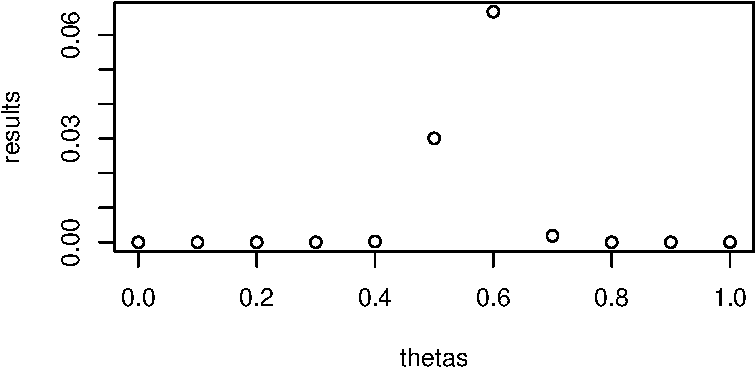
\includegraphics{hw2_602_files/figure-pdf/unnamed-chunk-1-1.pdf}

}

\end{figure}

c)

\[
p(\theta | \Sigma_{i=1}^{n}y_i = 57) = \frac{P(\Sigma_{i=1}^{n}y_i = 57 | \theta)P(\theta)}{P(\Sigma_{i=1}^{n}y_i = 57)}  \\
\text{each } P(\Theta = \theta) = \frac{1}{11}\\
\\
\]

sum function above\\
may need to add binomial coefficient and sum out the discrete values of
theta?

The posterior distribution and marginal distribution of Y are just
scaling constants since the denominator does not depend on theta and we
have equal belief for each of \(P(\theta)\).

\begin{Shaded}
\begin{Highlighting}[]
\NormalTok{marginal\_y }\OtherTok{=} \FunctionTok{sum}\NormalTok{((}\DecValTok{1}\SpecialCharTok{/}\DecValTok{11}\NormalTok{) }\SpecialCharTok{*} \FunctionTok{dbinom}\NormalTok{(}\DecValTok{57}\NormalTok{,}\DecValTok{100}\NormalTok{,thetas))}
\NormalTok{posterior }\OtherTok{=}\NormalTok{ (results }\SpecialCharTok{*}\NormalTok{ (}\DecValTok{1}\SpecialCharTok{/}\DecValTok{11}\NormalTok{))}\SpecialCharTok{/}\NormalTok{marginal\_y}
\FunctionTok{plot}\NormalTok{(thetas,posterior)}
\end{Highlighting}
\end{Shaded}

\begin{figure}[H]

{\centering 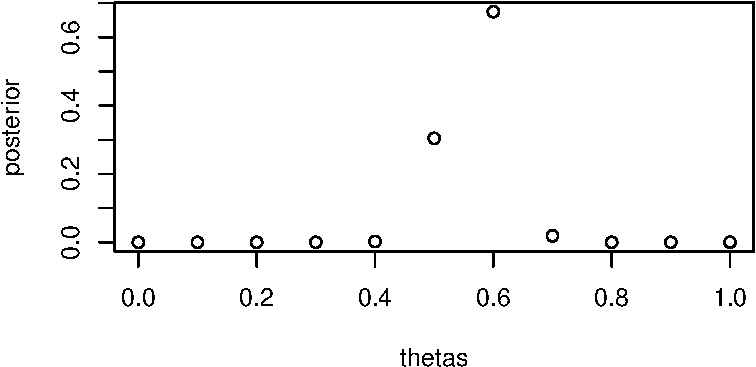
\includegraphics{hw2_602_files/figure-pdf/unnamed-chunk-2-1.pdf}

}

\end{figure}

d)

Not sure here on letting theta be any value in the interval.
Approximating that with discrete values below but not sure if that's
correct?

\begin{Shaded}
\begin{Highlighting}[]
\NormalTok{thetas }\OtherTok{=} \FunctionTok{seq}\NormalTok{(}\DecValTok{0}\NormalTok{,}\DecValTok{1}\NormalTok{,}\AttributeTok{by=}\FloatTok{0.001}\NormalTok{) }\CommentTok{\#U(0,1)}
\NormalTok{results }\OtherTok{=} \FunctionTok{dbinom}\NormalTok{(}\DecValTok{57}\NormalTok{,}\DecValTok{100}\NormalTok{,thetas)}
\FunctionTok{plot}\NormalTok{(thetas,results,}\AttributeTok{type=}\StringTok{"l"}\NormalTok{)}
\end{Highlighting}
\end{Shaded}

\begin{figure}[H]

{\centering 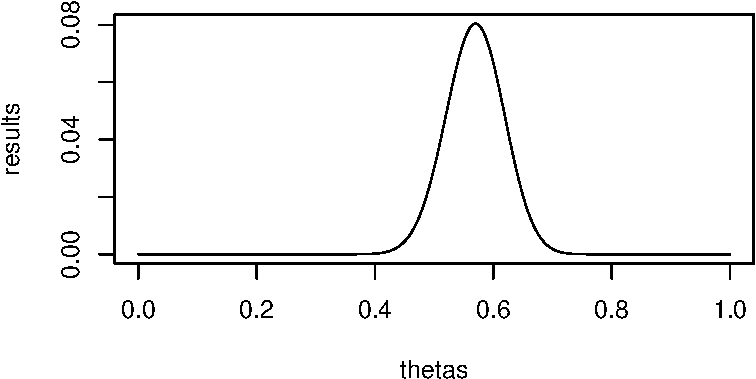
\includegraphics{hw2_602_files/figure-pdf/unnamed-chunk-3-1.pdf}

}

\end{figure}

e)

Same thing as d)

\begin{Shaded}
\begin{Highlighting}[]
\FunctionTok{plot}\NormalTok{(thetas,}\FunctionTok{dbeta}\NormalTok{(thetas,}\DecValTok{58}\NormalTok{,}\DecValTok{44}\NormalTok{),}\AttributeTok{type=}\StringTok{\textquotesingle{}l\textquotesingle{}}\NormalTok{)}
\end{Highlighting}
\end{Shaded}

\begin{figure}[H]

{\centering 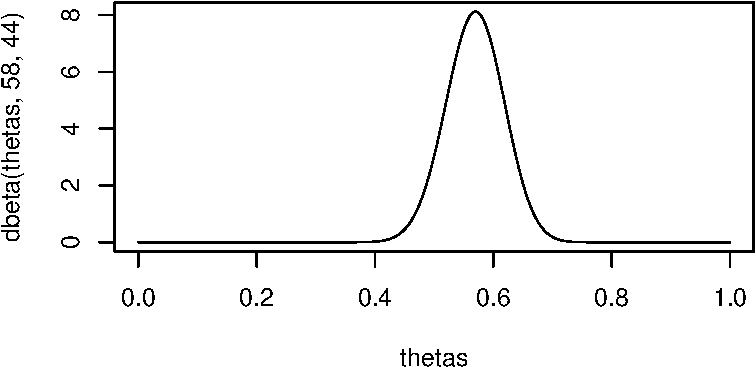
\includegraphics{hw2_602_files/figure-pdf/unnamed-chunk-4-1.pdf}

}

\end{figure}

\hypertarget{section-1}{%
\section{3.2}\label{section-1}}

Looks almost correct here but some kind of calculation is off?

\begin{Shaded}
\begin{Highlighting}[]
\NormalTok{theta0 }\OtherTok{=} \FunctionTok{seq}\NormalTok{(}\FloatTok{0.1}\NormalTok{,}\FloatTok{0.9}\NormalTok{,}\AttributeTok{by=}\FloatTok{0.1}\NormalTok{)}
\NormalTok{n0 }\OtherTok{=} \FunctionTok{c}\NormalTok{(}\DecValTok{1}\NormalTok{,}\DecValTok{2}\NormalTok{,}\DecValTok{8}\NormalTok{,}\DecValTok{16}\NormalTok{,}\DecValTok{32}\NormalTok{)}

\NormalTok{data}\OtherTok{=}\FunctionTok{c}\NormalTok{()}

\ControlFlowTok{for}\NormalTok{ (i }\ControlFlowTok{in}\NormalTok{ theta0) \{}
\ControlFlowTok{for}\NormalTok{ (j }\ControlFlowTok{in}\NormalTok{ n0) \{}
  
\NormalTok{    a }\OtherTok{=}\NormalTok{ i }\SpecialCharTok{*}\NormalTok{ j}
\NormalTok{    b }\OtherTok{=}\NormalTok{ (}\DecValTok{1}\SpecialCharTok{{-}}\NormalTok{i)}\SpecialCharTok{*}\NormalTok{j}

\NormalTok{    p }\OtherTok{=} \FunctionTok{pbeta}\NormalTok{(.}\DecValTok{5}\NormalTok{,a}\SpecialCharTok{+}\DecValTok{57}\NormalTok{,b}\SpecialCharTok{+}\DecValTok{43}\NormalTok{,}\AttributeTok{lower.tail=}\ConstantTok{FALSE}\NormalTok{) }\CommentTok{\#posterior (theta \textgreater{} .5 | sum = 57)}
\NormalTok{    data }\OtherTok{=} \FunctionTok{append}\NormalTok{(data,p)}

\NormalTok{\}}
\NormalTok{\}}

\NormalTok{probability\_data }\OtherTok{=} \FunctionTok{matrix}\NormalTok{(data,}\AttributeTok{nrow=}\DecValTok{9}\NormalTok{,}\AttributeTok{ncol=}\DecValTok{5}\NormalTok{,}\AttributeTok{byrow=}\ConstantTok{TRUE}\NormalTok{)}
\FunctionTok{contour}\NormalTok{(theta0,n0,probability\_data, }\AttributeTok{xlab=}\StringTok{"thetas"}\NormalTok{,}\AttributeTok{ylab=}\StringTok{\textquotesingle{}n0 values\textquotesingle{}}\NormalTok{)}
\end{Highlighting}
\end{Shaded}

\begin{figure}[H]

{\centering 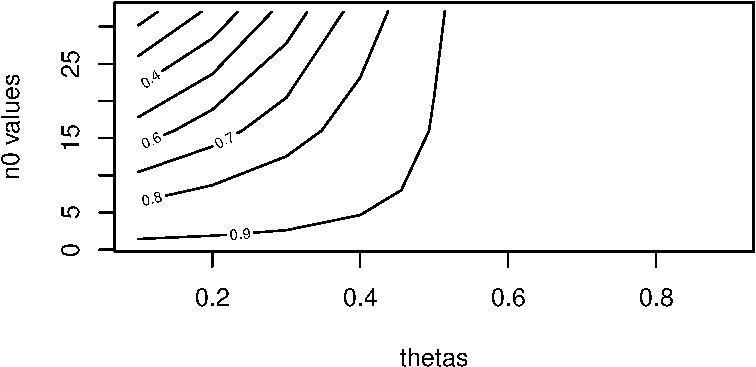
\includegraphics{hw2_602_files/figure-pdf/unnamed-chunk-5-1.pdf}

}

\end{figure}

\hypertarget{section-2}{%
\section{3.4}\label{section-2}}

\[
p(\theta | y) = \frac{p(y|\theta)p(\theta)}{p(y)}
\]

a)

for \(p(\theta|y)\) :

\begin{Shaded}
\begin{Highlighting}[]
\NormalTok{beta\_mean }\OtherTok{=} \ControlFlowTok{function}\NormalTok{(a,b)\{}
  \FunctionTok{print}\NormalTok{(}\StringTok{"mean:"}\NormalTok{)}
\NormalTok{  a }\SpecialCharTok{/}\NormalTok{ (a}\SpecialCharTok{+}\NormalTok{b)}
\NormalTok{\}}

\NormalTok{beta\_mode }\OtherTok{=} \ControlFlowTok{function}\NormalTok{(a,b)\{}
  \FunctionTok{print}\NormalTok{(}\StringTok{\textquotesingle{}mode:\textquotesingle{}}\NormalTok{)}
\NormalTok{  (a}\DecValTok{{-}1}\NormalTok{) }\SpecialCharTok{/}\NormalTok{ (a}\SpecialCharTok{+}\NormalTok{b}\DecValTok{{-}2}\NormalTok{)}
\NormalTok{\}}

\NormalTok{beta\_sd }\OtherTok{=} \ControlFlowTok{function}\NormalTok{(a,b)\{}
  \FunctionTok{print}\NormalTok{(}\StringTok{\textquotesingle{}standard deviation:\textquotesingle{}}\NormalTok{)}
\NormalTok{  var }\OtherTok{=}\NormalTok{ (a}\SpecialCharTok{*}\NormalTok{b) }\SpecialCharTok{/}\NormalTok{ ((a}\SpecialCharTok{+}\NormalTok{b)}\SpecialCharTok{\^{}}\DecValTok{2} \SpecialCharTok{*}\NormalTok{ (a}\SpecialCharTok{+}\NormalTok{b}\SpecialCharTok{+}\DecValTok{1}\NormalTok{))}
\NormalTok{  sd }\OtherTok{=} \FunctionTok{sqrt}\NormalTok{(var)}
  \FunctionTok{return}\NormalTok{(sd) }
\NormalTok{\}}

\NormalTok{CI\_28 }\OtherTok{=} \FunctionTok{c}\NormalTok{(}\FunctionTok{qbeta}\NormalTok{(.}\DecValTok{025}\NormalTok{,}\DecValTok{17}\NormalTok{,}\DecValTok{36}\NormalTok{),}\FunctionTok{qbeta}\NormalTok{(.}\DecValTok{975}\NormalTok{,}\DecValTok{17}\NormalTok{,}\DecValTok{36}\NormalTok{))}
\NormalTok{CI\_82 }\OtherTok{=} \FunctionTok{c}\NormalTok{(}\FunctionTok{qbeta}\NormalTok{(.}\DecValTok{025}\NormalTok{,}\DecValTok{23}\NormalTok{,}\DecValTok{30}\NormalTok{),}\FunctionTok{qbeta}\NormalTok{(.}\DecValTok{975}\NormalTok{,}\DecValTok{23}\NormalTok{,}\DecValTok{30}\NormalTok{))}

\CommentTok{\#data for the posterior w/ 2,8 prior and posterior a = 17, posterior b = 36}
\FunctionTok{print}\NormalTok{(}\StringTok{"using alpha = 17 and beta = 36 with beta(2,8) prior"}\NormalTok{)}
\end{Highlighting}
\end{Shaded}

\begin{verbatim}
[1] "using alpha = 17 and beta = 36 with beta(2,8) prior"
\end{verbatim}

\begin{Shaded}
\begin{Highlighting}[]
\FunctionTok{beta\_mean}\NormalTok{(}\DecValTok{17}\NormalTok{,}\DecValTok{36}\NormalTok{)}
\end{Highlighting}
\end{Shaded}

\begin{verbatim}
[1] "mean:"
\end{verbatim}

\begin{verbatim}
[1] 0.3207547
\end{verbatim}

\begin{Shaded}
\begin{Highlighting}[]
\FunctionTok{beta\_mode}\NormalTok{(}\DecValTok{17}\NormalTok{,}\DecValTok{36}\NormalTok{)}
\end{Highlighting}
\end{Shaded}

\begin{verbatim}
[1] "mode:"
\end{verbatim}

\begin{verbatim}
[1] 0.3137255
\end{verbatim}

\begin{Shaded}
\begin{Highlighting}[]
\FunctionTok{beta\_sd}\NormalTok{(}\DecValTok{17}\NormalTok{,}\DecValTok{36}\NormalTok{)}
\end{Highlighting}
\end{Shaded}

\begin{verbatim}
[1] "standard deviation:"
\end{verbatim}

\begin{verbatim}
[1] 0.0635189
\end{verbatim}

\begin{Shaded}
\begin{Highlighting}[]
\FunctionTok{print}\NormalTok{(}\FunctionTok{c}\NormalTok{(}\StringTok{"95\% CI"}\NormalTok{,CI\_28))}
\end{Highlighting}
\end{Shaded}

\begin{verbatim}
[1] "95% CI"            "0.203297787819103" "0.451023982216632"
\end{verbatim}

\begin{Shaded}
\begin{Highlighting}[]
\CommentTok{\#with 8,2 prior }
\FunctionTok{print}\NormalTok{(}\StringTok{" "}\NormalTok{)}
\end{Highlighting}
\end{Shaded}

\begin{verbatim}
[1] " "
\end{verbatim}

\begin{Shaded}
\begin{Highlighting}[]
\FunctionTok{print}\NormalTok{(}\StringTok{"================================================"}\NormalTok{)}
\end{Highlighting}
\end{Shaded}

\begin{verbatim}
[1] "================================================"
\end{verbatim}

\begin{Shaded}
\begin{Highlighting}[]
\FunctionTok{print}\NormalTok{(}\StringTok{"using alpha = 23, beta = 30 with beta(8,2) prior"}\NormalTok{)}
\end{Highlighting}
\end{Shaded}

\begin{verbatim}
[1] "using alpha = 23, beta = 30 with beta(8,2) prior"
\end{verbatim}

\begin{Shaded}
\begin{Highlighting}[]
\FunctionTok{beta\_mean}\NormalTok{(}\DecValTok{23}\NormalTok{,}\DecValTok{30}\NormalTok{)}
\end{Highlighting}
\end{Shaded}

\begin{verbatim}
[1] "mean:"
\end{verbatim}

\begin{verbatim}
[1] 0.4339623
\end{verbatim}

\begin{Shaded}
\begin{Highlighting}[]
\FunctionTok{beta\_mode}\NormalTok{(}\DecValTok{23}\NormalTok{,}\DecValTok{30}\NormalTok{)}
\end{Highlighting}
\end{Shaded}

\begin{verbatim}
[1] "mode:"
\end{verbatim}

\begin{verbatim}
[1] 0.4313725
\end{verbatim}

\begin{Shaded}
\begin{Highlighting}[]
\FunctionTok{beta\_sd}\NormalTok{(}\DecValTok{23}\NormalTok{,}\DecValTok{30}\NormalTok{)}
\end{Highlighting}
\end{Shaded}

\begin{verbatim}
[1] "standard deviation:"
\end{verbatim}

\begin{verbatim}
[1] 0.06744532
\end{verbatim}

\begin{Shaded}
\begin{Highlighting}[]
\FunctionTok{print}\NormalTok{(}\FunctionTok{c}\NormalTok{(}\StringTok{"95\% CI"}\NormalTok{,CI\_82))}
\end{Highlighting}
\end{Shaded}

\begin{verbatim}
[1] "95% CI"            "0.304695624711747" "0.567952795996458"
\end{verbatim}

Confidence interval is calculated below and plotted

\begin{Shaded}
\begin{Highlighting}[]
\CommentTok{\#plotting prior p(\textbackslash{}theta)}
\NormalTok{thetas }\OtherTok{=} \FunctionTok{seq}\NormalTok{(}\DecValTok{0}\NormalTok{,}\DecValTok{1}\NormalTok{,}\AttributeTok{by=}\FloatTok{0.001}\NormalTok{) }\CommentTok{\#U(0,1)}

\FunctionTok{plot}\NormalTok{(thetas, }\FunctionTok{dbeta}\NormalTok{(thetas, }\DecValTok{2}\NormalTok{,}\DecValTok{8}\NormalTok{), }\AttributeTok{type=}\StringTok{\textquotesingle{}l\textquotesingle{}}\NormalTok{,}\AttributeTok{main=}\StringTok{"p(theta)"}\NormalTok{)}
\end{Highlighting}
\end{Shaded}

\begin{figure}[H]

{\centering 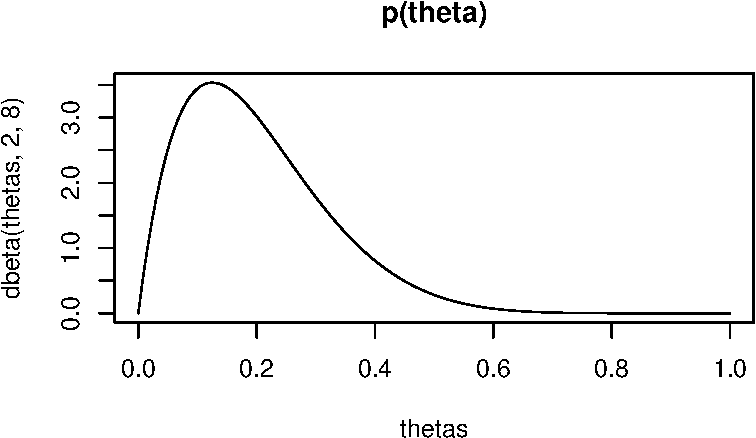
\includegraphics{hw2_602_files/figure-pdf/unnamed-chunk-7-1.pdf}

}

\end{figure}

\begin{Shaded}
\begin{Highlighting}[]
\CommentTok{\#plotting p(y=15|\textbackslash{}theta)}
\CommentTok{\#plot a binomial here }
\FunctionTok{plot}\NormalTok{(thetas, }\FunctionTok{dbinom}\NormalTok{(}\DecValTok{15}\NormalTok{,}\DecValTok{43}\NormalTok{,thetas))}
\end{Highlighting}
\end{Shaded}

\begin{figure}[H]

{\centering 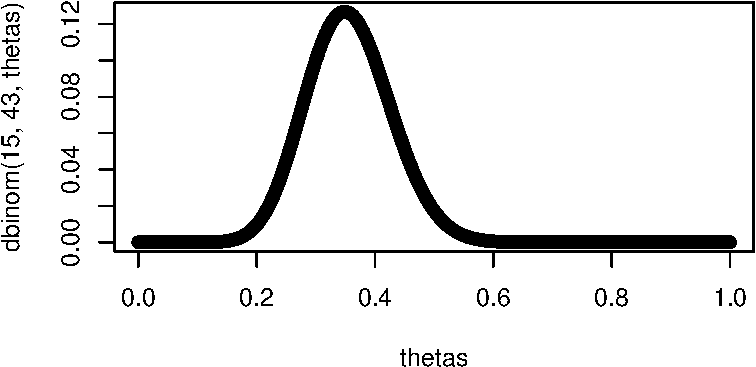
\includegraphics{hw2_602_files/figure-pdf/unnamed-chunk-7-2.pdf}

}

\end{figure}

\begin{Shaded}
\begin{Highlighting}[]
\CommentTok{\#posterior which is beta(2 + success, 8 + failure) = beta()}
\NormalTok{a}\OtherTok{=}\DecValTok{2}\SpecialCharTok{+}\DecValTok{15}
\NormalTok{b}\OtherTok{=}\DecValTok{8}\SpecialCharTok{+}\DecValTok{28}
\FunctionTok{plot}\NormalTok{(thetas, }\FunctionTok{dbeta}\NormalTok{(thetas,a,b),}\AttributeTok{type=}\StringTok{\textquotesingle{}l\textquotesingle{}}\NormalTok{,}\AttributeTok{main=}\StringTok{"posterior model"}\NormalTok{)}
\FunctionTok{abline}\NormalTok{(}\AttributeTok{v=}\FunctionTok{beta\_mean}\NormalTok{(a,b), }\AttributeTok{col=}\StringTok{\textquotesingle{}red\textquotesingle{}}\NormalTok{) }\CommentTok{\#mean}
\end{Highlighting}
\end{Shaded}

\begin{verbatim}
[1] "mean:"
\end{verbatim}

\begin{Shaded}
\begin{Highlighting}[]
\FunctionTok{abline}\NormalTok{(}\AttributeTok{v=}\FunctionTok{beta\_mode}\NormalTok{(a,b), }\AttributeTok{col=}\StringTok{\textquotesingle{}blue\textquotesingle{}}\NormalTok{) }\CommentTok{\#mode}
\end{Highlighting}
\end{Shaded}

\begin{verbatim}
[1] "mode:"
\end{verbatim}

\begin{Shaded}
\begin{Highlighting}[]
\CommentTok{\# CI }
\FunctionTok{abline}\NormalTok{(}\AttributeTok{v=}\FunctionTok{qbeta}\NormalTok{(.}\DecValTok{975}\NormalTok{,a,b),}\AttributeTok{col=}\StringTok{\textquotesingle{}green\textquotesingle{}}\NormalTok{) }\CommentTok{\#lower bound }
\FunctionTok{abline}\NormalTok{(}\AttributeTok{v=}\FunctionTok{qbeta}\NormalTok{(.}\DecValTok{025}\NormalTok{,a,b),}\AttributeTok{col=}\StringTok{\textquotesingle{}green\textquotesingle{}}\NormalTok{) }\CommentTok{\#upper bound }
\end{Highlighting}
\end{Shaded}

\begin{figure}[H]

{\centering 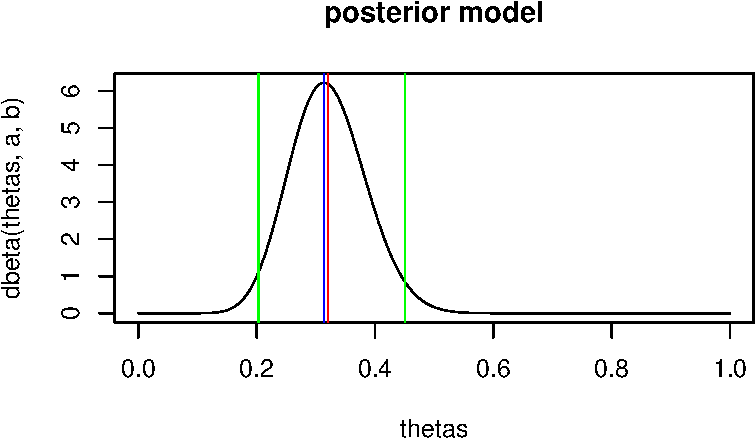
\includegraphics{hw2_602_files/figure-pdf/unnamed-chunk-7-3.pdf}

}

\end{figure}



\end{document}
